\documentclass[a4paper]{article}
\usepackage{geometry}
\usepackage{multicol}
\usepackage{graphicx}
\geometry{margin=0.25in}

\begin{document}
\begin{multicols}{3}
\raggedright
\fontsize{6pt}{0.3pt}\selectfont
\setlength{\abovedisplayskip}{2pt}
\setlength{\belowdisplayskip}{0pt}

Maybe there is something here 
not again

% \begin{minipage}{0.31\textwidth}
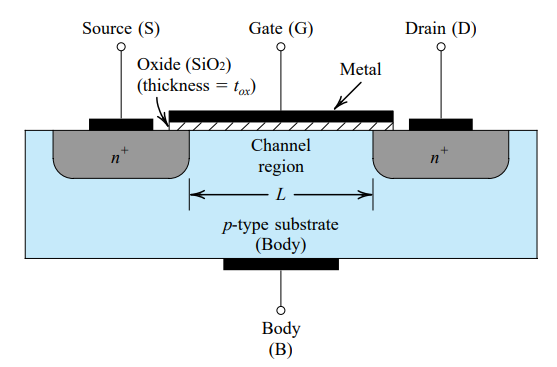
\includegraphics[width=\linewidth]{imgs/nmos}
The size of the "process" indicates the minimum
possible channel length. 

Magnitude of the electron charge in the channel [Q]:$$|Q|=C_{OX}(WL)v_{OV}$$
$C_{OX}$ is the oxide capacitance, [F/m$^2$]

$$C_{OX}=\frac{\epsilon_{OX}}{t_{OX}}$$

$\epsilon_{OX}$ is the permittivity of the SiO$_2$.\\
$t_{OX}$ is the oxide thickness.

For $C_{OX}$ per micron squared, use \\
$C=C_{OX}WL$ [fF]

$$i_D=\left[ (\mu_nC_{OX})\left(\frac{W}{L}\right)(v_{GS}-V_t)\right]v_{DS}$$
$$i_D=\left[ g_{DS} \right]v_{DS}$$
$$k_n^{'}=\mu_nC_{OX}$$
$$k_n=k_n^{'}(W/L)$$

When $V_{DS}$ is small, the MOSFET behaves as a linear 
resistance $r_{DS}$ whose value is controlled by the gate 
voltage $v_{GS}$.
$$r_{DS}=\frac{1}{g_{DS}}$$

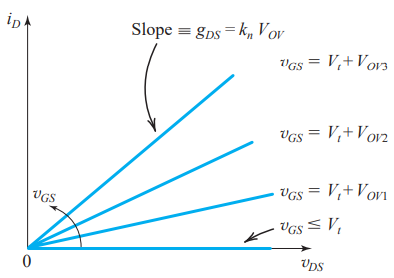
\includegraphics[width=\linewidth]{imgs/nmos_as_r}

\hrule
\vspace{1mm}
Triode vs Saturation

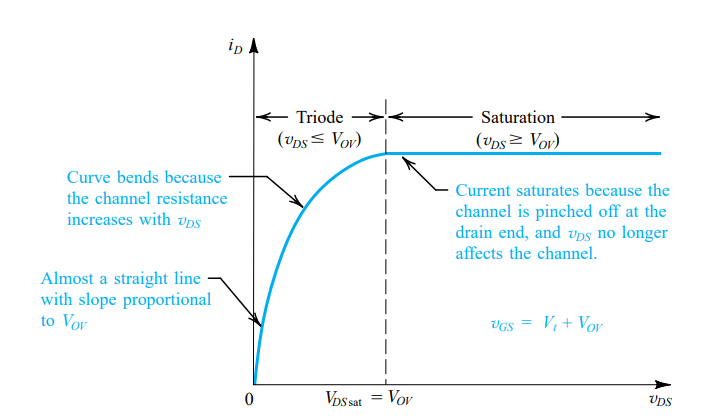
\includegraphics[width=\linewidth]{imgs/triode_sat.png}

Triode ($v_{DS} \leq V_{OV}$)

$$i_D=k_n^{'}\left(\frac{W}{L}\right)\left(V_{OV}-\frac{1}{2}v_{DS}\right)v_{DS}$$
$$i_D=k_n^{'}\left(\frac{W}{L}\right)\left[(v_{GS}-V_t)v_{DS}-\frac{1}{2}v_{DS}^2\right]$$

Saturation ($v_{DS} \geq V_{OV}$)

$$i_D=\frac{1}{2}k_n^{'}\left(\frac{W}{L}\right)V_{OV}^2$$

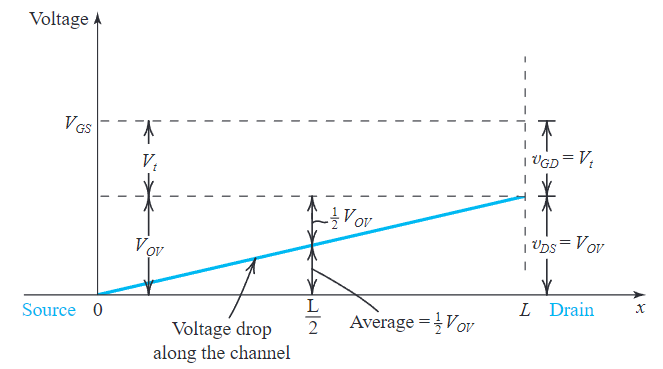
\includegraphics[width=\linewidth]{imgs/mosfet_sat.png}

Constant $V_{OV}$ can be replaced by variable $v_{OV}$.

PMOS transistors operate similarly but the polarity is
reversed, so $v_{GS}$ must be negative and larger than 
a negative $v_{tp}$, as is $v_{DS}$ negative.

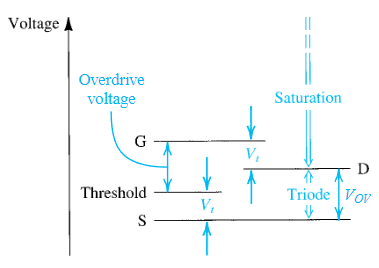
\includegraphics[width=\linewidth]{imgs/mosfet_operation.png}

If you care about \textbf{channel-length modulation}, then use
the expression:
$$i_D=\frac{1}{2}k_n^{'}\left(\frac{W}{L}\right)(v_{GS}-V_{th})^2(1+\lambda v_{DS})$$

$v_{DS}=-\frac{1}{\lambda} \mid$
$V_A=\frac{1}{\lambda} \mid$
$V_A=V_A^{'}L$  

$V_A$ has units of volts.\\
$V_A^{'}$ has units of volts per micron.

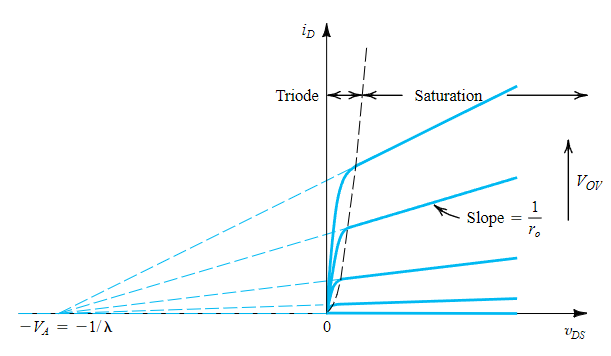
\includegraphics[width=\linewidth]{imgs/va_mosfet.png}


% \end{minipage}
% \begin{minipage}{0.31\textwidth}
%     More text over here
% \end{minipage}

\end{multicols}
\end{document}